\documentclass[12pt]{article}
\usepackage[table]{xcolor}
\usepackage[shortlabels]{enumitem}
\usepackage{tabularx,xltabular}
\usepackage{graphicx}
\usepackage{hyperref}
\usepackage{verbatim}
\usepackage{geometry}
\usepackage{ulem}
\usepackage[official]{eurosym}
\usepackage{tikz}
\usetikzlibrary{arrows,backgrounds,calc,decorations.markings,patterns,3d}
\usepackage{pgfplots}
\pgfplotsset{compat = newest}
\usetikzlibrary{fit}
\newcommand\addvmargin[1]{
\usetikzlibrary{arrows}
\node[fit=(current bounding box),inner ysep=#1,inner xsep=0]{};}
\usepackage{cancel}
\usepackage{fontspec}
\usepackage{array}  
\geometry{a4paper, top=2cm, left=2cm, right=2cm, bottom=2cm, headsep=1cm}
\usepackage{tabu}
\usepackage{pst-node}
\usepackage{colortbl}
\usepackage{array}
\usepackage{german}
\setlength\parindent{0pt}
\newcolumntype{?}{!{\vrule width 1pt}}
\usepackage{makecell}
\renewcommand{\arraystretch}{2.5}
\usepackage{pbox}
\usepackage{amssymb}
\usepackage{amsmath}
\usepackage{booktabs}
\newcolumntype{L}[1]{>{\raggedright\let\newline\\\arraybackslash\hspace{0pt}}m{#1}}
\newcolumntype{C}[1]{>{\centering\let\newline\\\arraybackslash\hspace{0pt}}m{#1}}
\newcolumntype{R}[1]{>{\raggedleft\let\newline\\\arraybackslash\hspace{0pt}}m{#1}}
\begin{document}
\rightline{Datum: 08.06.2023}
\centerline{{\Large Tägliche Übungen}} 
\vspace{1cm}
\noindent \\


\begin{xltabular}{\textwidth}{|C{0.75cm}|X|C{0.75cm}|X|}
\arrayrulecolor{black}\hline
a)&$\begin{aligned}
 a=&-11~ \rightarrow ~ 3 \cdot a + 2 \cdot a=?
\end{aligned}$
&
b)&$\begin{aligned}
 x=&-11~ \rightarrow ~ 3 \cdot x + 1=?
\end{aligned}$
\\\hline
c)&$\begin{aligned}
 a=&11~ \rightarrow ~ 2 \cdot a + 3 \cdot a=?
\end{aligned}$
&
d)&$\begin{aligned}
 z=&-1~ \rightarrow ~ 2 \cdot z + 3=?
\end{aligned}$
\\\hline
e)&$x+24 = 4$
&
f)&$a+35 = 32$
\\\hline
g)&$a+28 = 32$
&
h)&$a-3 = 49$
\\\hline
i)&$x+44 = 37$
&
j)&$b-5 = 49$
\\\hline
k)&$x+18 = 38$
&
l)&$b-18 = 50$
\\\hline
m)&$x-12 = 32$
&
n)&$b+34 = 8$
\\\hline
o)&$x+42 = 13$
&
p)&$y-29 = 50$
\\\hline
q)&$b+7 = 2$
&
r)&$a+32 = 11$
\\\hline
s)&$x-49 = 27$
&
t)&$x-40 = 45$
\\\hline
u)&$a-17 = 34$
&
v)&$x-28 = 1$
\\\hline
w)&$a+3 = 24$
&
x)&$b+2 = 13$
\\\hline
y)&$a+46 = 28$
&
z)&$x+9 = 10$
\\\hline
\end{xltabular}
\vspace{0.5cm}
\newpage
\rightline{Datum: 08.06.2023}
\centerline{{\large Lösungen Tägliche Übungen}} 
\vspace{0.5cm}

\begin{xltabular}{\textwidth}{|C{0.75cm}|X|C{0.75cm}|X|}
\arrayrulecolor{black}\hline
a)&$\begin{aligned}
\textcolor{red}{a=-11} & \rightarrow\\
3 \cdot a + 2 \cdot a=&3 \cdot \textcolor{red}{(-11)} + 2 \cdot \textcolor{red}{(-11)}=-55\\
\end{aligned}$
&
b)&$\begin{aligned}
\textcolor{red}{x=-11} & \rightarrow\\
3 \cdot x + 1=&3 \cdot \textcolor{red}{(-11)} + 1=-32\\
\end{aligned}$
\\\hline
c)&$\begin{aligned}
\textcolor{red}{a=11} & \rightarrow\\
2 \cdot a + 3 \cdot a=&2 \cdot \textcolor{red}{11} + 3 \cdot \textcolor{red}{11}=55\\
\end{aligned}$
&
d)&$\begin{aligned}
\textcolor{red}{z=-1} & \rightarrow\\
2 \cdot z + 3=&2 \cdot \textcolor{red}{(-1)} + 3=1\\
\end{aligned}$
\\\hline
e)&\begingroup\setlength{\jot}{-0.03cm}
\tikzstyle{background grid}=[draw, black!15,step=.5cm]
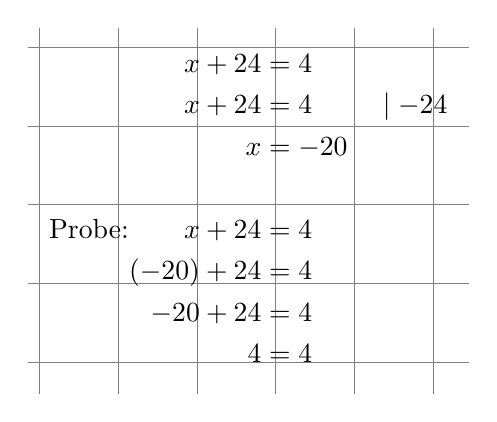
\begin{tikzpicture}[show background grid]
\node[below right] at (0,0.1) {
$\begin{aligned}
x+24  &= 4& &  \\
x + 24 &=4& & \mid - 24\\
x &=-20& & 
\\
\\
\mbox{Probe:}\qquad x+24  &= 4& &  \\
\left(-20\right)+24  &= 4& &  \\
-20+24 &=4& &  \\
4 &=4& &  \\
\end{aligned}$};
\end{tikzpicture}
\endgroup
&
f)&\begingroup\setlength{\jot}{-0.03cm}
\tikzstyle{background grid}=[draw, black!15,step=.5cm]
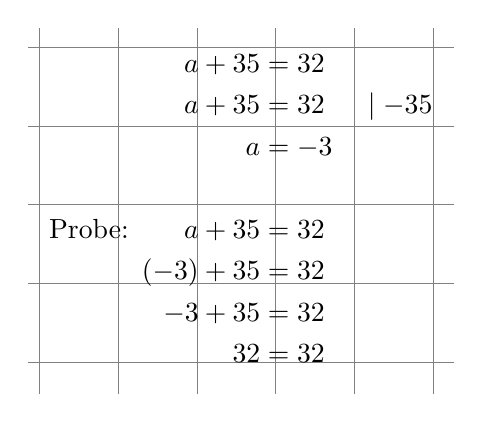
\begin{tikzpicture}[show background grid]
\node[below right] at (0,0.1) {
$\begin{aligned}
a+35  &= 32& &  \\
a + 35 &=32& & \mid - 35\\
a &=-3& & 
\\
\\
\mbox{Probe:}\qquad a+35  &= 32& &  \\
\left(-3\right)+35  &= 32& &  \\
-3+35 &=32& &  \\
32 &=32& &  \\
\end{aligned}$};
\end{tikzpicture}
\endgroup
\\\hline
g)&\begingroup\setlength{\jot}{-0.03cm}
\tikzstyle{background grid}=[draw, black!15,step=.5cm]
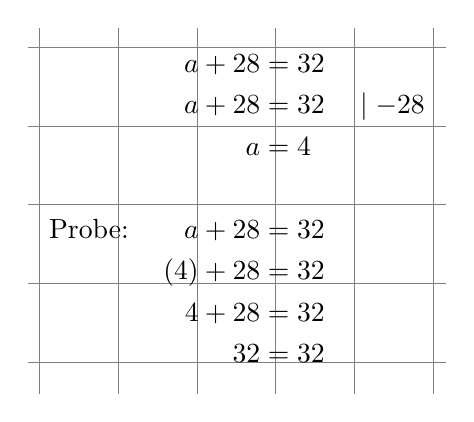
\begin{tikzpicture}[show background grid]
\node[below right] at (0,0.1) {
$\begin{aligned}
a+28  &= 32& &  \\
a + 28 &=32& & \mid - 28\\
a &=4& & 
\\
\\
\mbox{Probe:}\qquad a+28  &= 32& &  \\
\left(4\right)+28  &= 32& &  \\
4+28 &=32& &  \\
32 &=32& &  \\
\end{aligned}$};
\end{tikzpicture}
\endgroup
&
h)&\begingroup\setlength{\jot}{-0.03cm}
\tikzstyle{background grid}=[draw, black!15,step=.5cm]
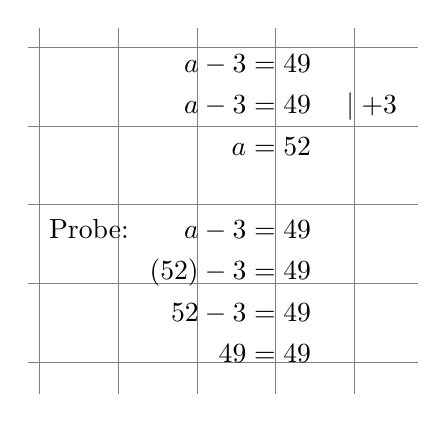
\begin{tikzpicture}[show background grid]
\node[below right] at (0,0.1) {
$\begin{aligned}
a-3  &= 49& &  \\
a - 3 &=49& & \mid + 3\\
a &=52& & 
\\
\\
\mbox{Probe:}\qquad a-3  &= 49& &  \\
\left(52\right)-3  &= 49& &  \\
52-3 &=49& &  \\
49 &=49& &  \\
\end{aligned}$};
\end{tikzpicture}
\endgroup
\\\hline
i)&\begingroup\setlength{\jot}{-0.03cm}
\tikzstyle{background grid}=[draw, black!15,step=.5cm]
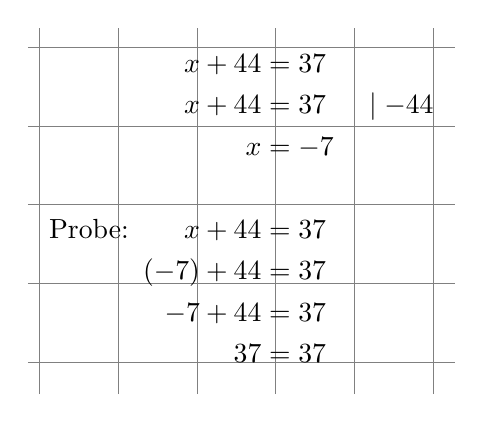
\begin{tikzpicture}[show background grid]
\node[below right] at (0,0.1) {
$\begin{aligned}
x+44  &= 37& &  \\
x + 44 &=37& & \mid - 44\\
x &=-7& & 
\\
\\
\mbox{Probe:}\qquad x+44  &= 37& &  \\
\left(-7\right)+44  &= 37& &  \\
-7+44 &=37& &  \\
37 &=37& &  \\
\end{aligned}$};
\end{tikzpicture}
\endgroup
&
j)&\begingroup\setlength{\jot}{-0.03cm}
\tikzstyle{background grid}=[draw, black!15,step=.5cm]
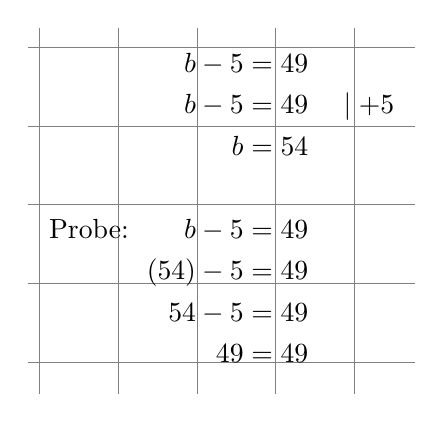
\begin{tikzpicture}[show background grid]
\node[below right] at (0,0.1) {
$\begin{aligned}
b-5  &= 49& &  \\
b - 5 &=49& & \mid + 5\\
b &=54& & 
\\
\\
\mbox{Probe:}\qquad b-5  &= 49& &  \\
\left(54\right)-5  &= 49& &  \\
54-5 &=49& &  \\
49 &=49& &  \\
\end{aligned}$};
\end{tikzpicture}
\endgroup
\\\hline
k)&\begingroup\setlength{\jot}{-0.03cm}
\tikzstyle{background grid}=[draw, black!15,step=.5cm]
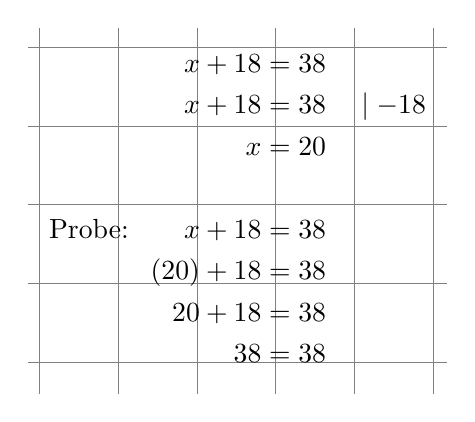
\begin{tikzpicture}[show background grid]
\node[below right] at (0,0.1) {
$\begin{aligned}
x+18  &= 38& &  \\
x + 18 &=38& & \mid - 18\\
x &=20& & 
\\
\\
\mbox{Probe:}\qquad x+18  &= 38& &  \\
\left(20\right)+18  &= 38& &  \\
20+18 &=38& &  \\
38 &=38& &  \\
\end{aligned}$};
\end{tikzpicture}
\endgroup
&
l)&\begingroup\setlength{\jot}{-0.03cm}
\tikzstyle{background grid}=[draw, black!15,step=.5cm]
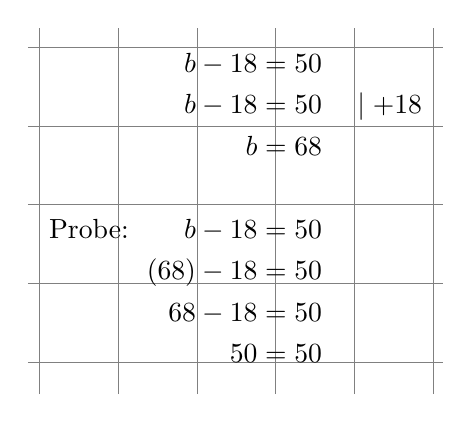
\begin{tikzpicture}[show background grid]
\node[below right] at (0,0.1) {
$\begin{aligned}
b-18  &= 50& &  \\
b - 18 &=50& & \mid + 18\\
b &=68& & 
\\
\\
\mbox{Probe:}\qquad b-18  &= 50& &  \\
\left(68\right)-18  &= 50& &  \\
68-18 &=50& &  \\
50 &=50& &  \\
\end{aligned}$};
\end{tikzpicture}
\endgroup
\\\hline
m)&\begingroup\setlength{\jot}{-0.03cm}
\tikzstyle{background grid}=[draw, black!15,step=.5cm]
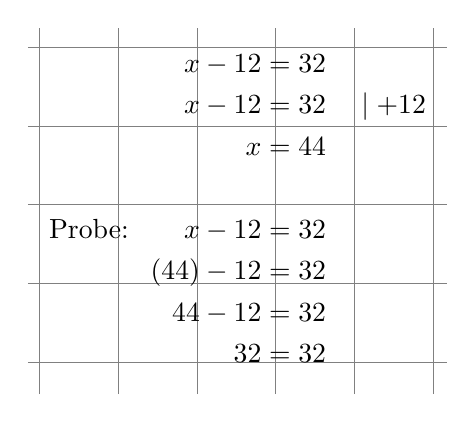
\begin{tikzpicture}[show background grid]
\node[below right] at (0,0.1) {
$\begin{aligned}
x-12  &= 32& &  \\
x - 12 &=32& & \mid + 12\\
x &=44& & 
\\
\\
\mbox{Probe:}\qquad x-12  &= 32& &  \\
\left(44\right)-12  &= 32& &  \\
44-12 &=32& &  \\
32 &=32& &  \\
\end{aligned}$};
\end{tikzpicture}
\endgroup
&
n)&\begingroup\setlength{\jot}{-0.03cm}
\tikzstyle{background grid}=[draw, black!15,step=.5cm]
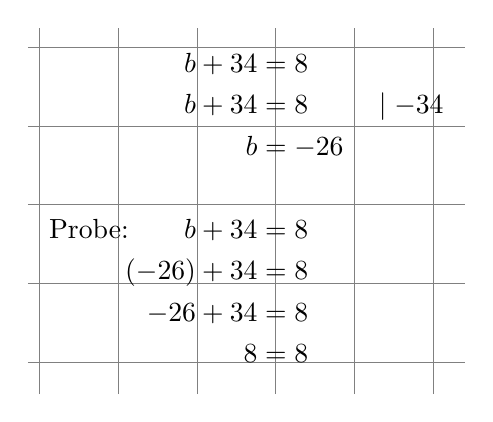
\begin{tikzpicture}[show background grid]
\node[below right] at (0,0.1) {
$\begin{aligned}
b+34  &= 8& &  \\
b + 34 &=8& & \mid - 34\\
b &=-26& & 
\\
\\
\mbox{Probe:}\qquad b+34  &= 8& &  \\
\left(-26\right)+34  &= 8& &  \\
-26+34 &=8& &  \\
8 &=8& &  \\
\end{aligned}$};
\end{tikzpicture}
\endgroup
\\\hline
o)&\begingroup\setlength{\jot}{-0.03cm}
\tikzstyle{background grid}=[draw, black!15,step=.5cm]
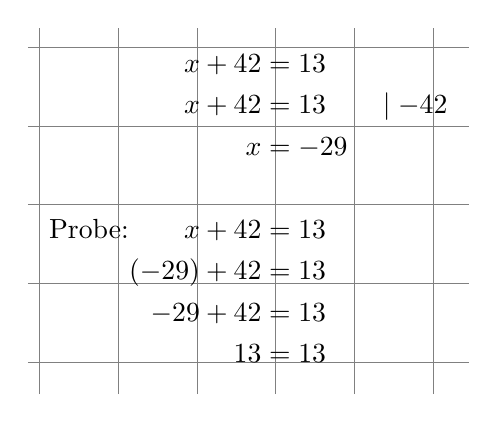
\begin{tikzpicture}[show background grid]
\node[below right] at (0,0.1) {
$\begin{aligned}
x+42  &= 13& &  \\
x + 42 &=13& & \mid - 42\\
x &=-29& & 
\\
\\
\mbox{Probe:}\qquad x+42  &= 13& &  \\
\left(-29\right)+42  &= 13& &  \\
-29+42 &=13& &  \\
13 &=13& &  \\
\end{aligned}$};
\end{tikzpicture}
\endgroup
&
p)&\begingroup\setlength{\jot}{-0.03cm}
\tikzstyle{background grid}=[draw, black!15,step=.5cm]
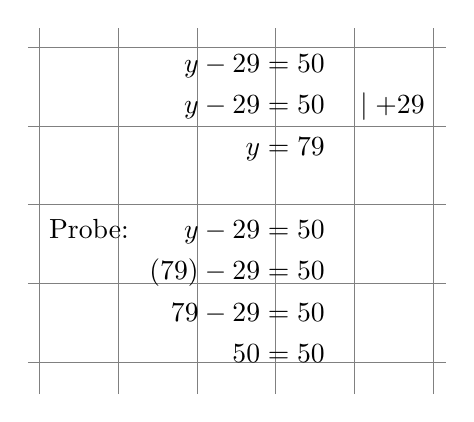
\begin{tikzpicture}[show background grid]
\node[below right] at (0,0.1) {
$\begin{aligned}
y-29  &= 50& &  \\
y - 29 &=50& & \mid + 29\\
y &=79& & 
\\
\\
\mbox{Probe:}\qquad y-29  &= 50& &  \\
\left(79\right)-29  &= 50& &  \\
79-29 &=50& &  \\
50 &=50& &  \\
\end{aligned}$};
\end{tikzpicture}
\endgroup
\\\hline
q)&\begingroup\setlength{\jot}{-0.03cm}
\tikzstyle{background grid}=[draw, black!15,step=.5cm]
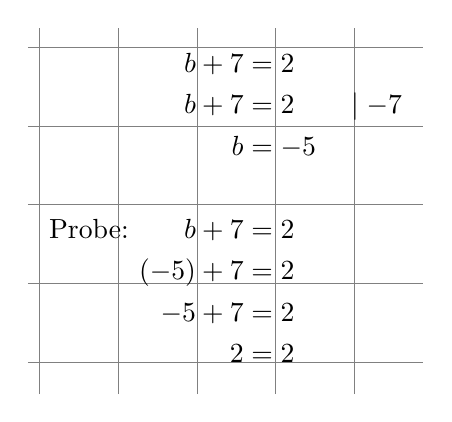
\begin{tikzpicture}[show background grid]
\node[below right] at (0,0.1) {
$\begin{aligned}
b+7  &= 2& &  \\
b + 7 &=2& & \mid - 7\\
b &=-5& & 
\\
\\
\mbox{Probe:}\qquad b+7  &= 2& &  \\
\left(-5\right)+7  &= 2& &  \\
-5+7 &=2& &  \\
2 &=2& &  \\
\end{aligned}$};
\end{tikzpicture}
\endgroup
&
r)&\begingroup\setlength{\jot}{-0.03cm}
\tikzstyle{background grid}=[draw, black!15,step=.5cm]
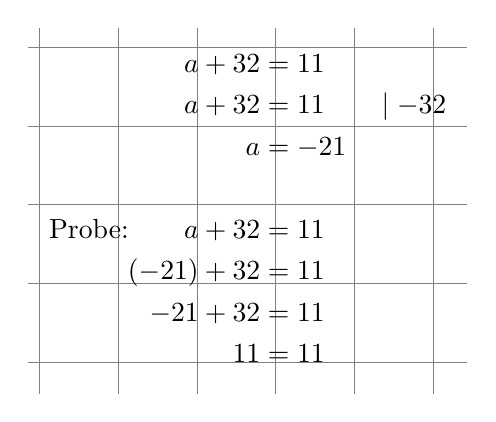
\begin{tikzpicture}[show background grid]
\node[below right] at (0,0.1) {
$\begin{aligned}
a+32  &= 11& &  \\
a + 32 &=11& & \mid - 32\\
a &=-21& & 
\\
\\
\mbox{Probe:}\qquad a+32  &= 11& &  \\
\left(-21\right)+32  &= 11& &  \\
-21+32 &=11& &  \\
11 &=11& &  \\
\end{aligned}$};
\end{tikzpicture}
\endgroup
\\\hline
s)&\begingroup\setlength{\jot}{-0.03cm}
\tikzstyle{background grid}=[draw, black!15,step=.5cm]
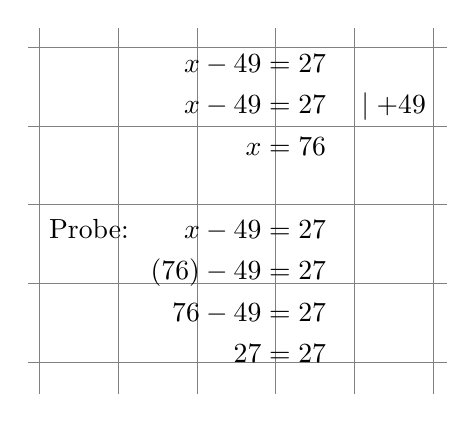
\begin{tikzpicture}[show background grid]
\node[below right] at (0,0.1) {
$\begin{aligned}
x-49  &= 27& &  \\
x - 49 &=27& & \mid + 49\\
x &=76& & 
\\
\\
\mbox{Probe:}\qquad x-49  &= 27& &  \\
\left(76\right)-49  &= 27& &  \\
76-49 &=27& &  \\
27 &=27& &  \\
\end{aligned}$};
\end{tikzpicture}
\endgroup
&
t)&\begingroup\setlength{\jot}{-0.03cm}
\tikzstyle{background grid}=[draw, black!15,step=.5cm]
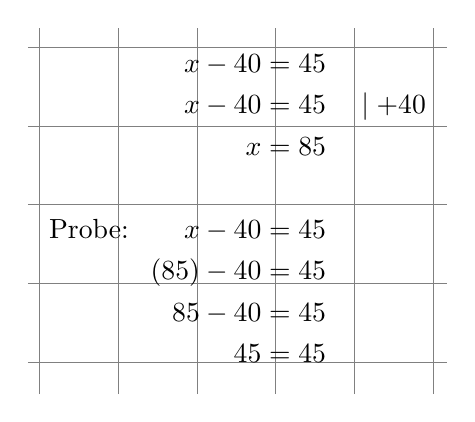
\begin{tikzpicture}[show background grid]
\node[below right] at (0,0.1) {
$\begin{aligned}
x-40  &= 45& &  \\
x - 40 &=45& & \mid + 40\\
x &=85& & 
\\
\\
\mbox{Probe:}\qquad x-40  &= 45& &  \\
\left(85\right)-40  &= 45& &  \\
85-40 &=45& &  \\
45 &=45& &  \\
\end{aligned}$};
\end{tikzpicture}
\endgroup
\\\hline
u)&\begingroup\setlength{\jot}{-0.03cm}
\tikzstyle{background grid}=[draw, black!15,step=.5cm]
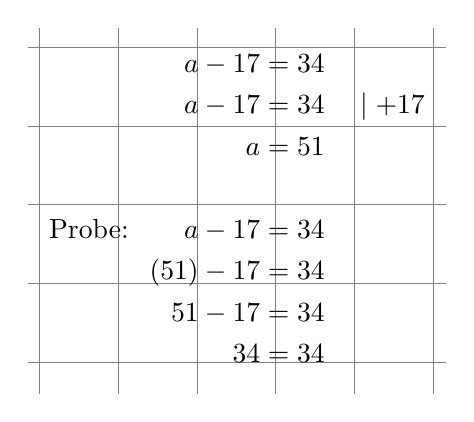
\begin{tikzpicture}[show background grid]
\node[below right] at (0,0.1) {
$\begin{aligned}
a-17  &= 34& &  \\
a - 17 &=34& & \mid + 17\\
a &=51& & 
\\
\\
\mbox{Probe:}\qquad a-17  &= 34& &  \\
\left(51\right)-17  &= 34& &  \\
51-17 &=34& &  \\
34 &=34& &  \\
\end{aligned}$};
\end{tikzpicture}
\endgroup
&
v)&\begingroup\setlength{\jot}{-0.03cm}
\tikzstyle{background grid}=[draw, black!15,step=.5cm]
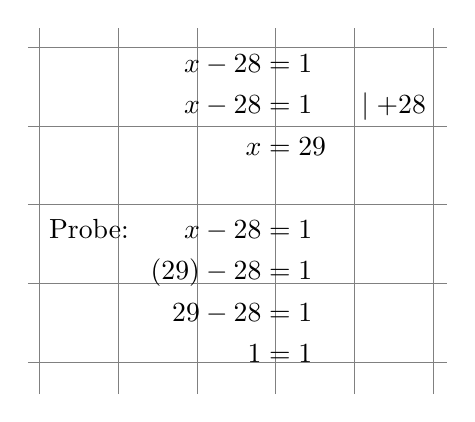
\begin{tikzpicture}[show background grid]
\node[below right] at (0,0.1) {
$\begin{aligned}
x-28  &= 1& &  \\
x - 28 &=1& & \mid + 28\\
x &=29& & 
\\
\\
\mbox{Probe:}\qquad x-28  &= 1& &  \\
\left(29\right)-28  &= 1& &  \\
29-28 &=1& &  \\
1 &=1& &  \\
\end{aligned}$};
\end{tikzpicture}
\endgroup
\\\hline
w)&\begingroup\setlength{\jot}{-0.03cm}
\tikzstyle{background grid}=[draw, black!15,step=.5cm]
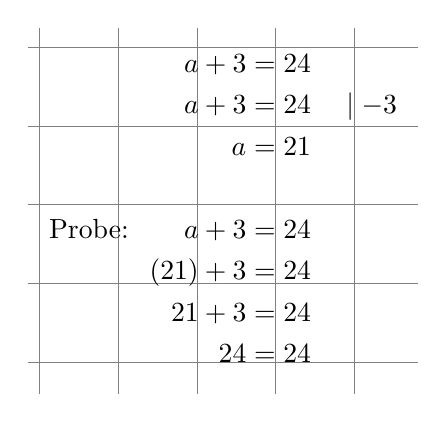
\begin{tikzpicture}[show background grid]
\node[below right] at (0,0.1) {
$\begin{aligned}
a+3  &= 24& &  \\
a + 3 &=24& & \mid - 3\\
a &=21& & 
\\
\\
\mbox{Probe:}\qquad a+3  &= 24& &  \\
\left(21\right)+3  &= 24& &  \\
21+3 &=24& &  \\
24 &=24& &  \\
\end{aligned}$};
\end{tikzpicture}
\endgroup
&
x)&\begingroup\setlength{\jot}{-0.03cm}
\tikzstyle{background grid}=[draw, black!15,step=.5cm]
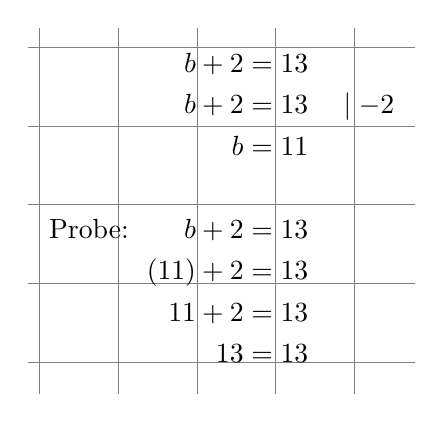
\begin{tikzpicture}[show background grid]
\node[below right] at (0,0.1) {
$\begin{aligned}
b+2  &= 13& &  \\
b + 2 &=13& & \mid - 2\\
b &=11& & 
\\
\\
\mbox{Probe:}\qquad b+2  &= 13& &  \\
\left(11\right)+2  &= 13& &  \\
11+2 &=13& &  \\
13 &=13& &  \\
\end{aligned}$};
\end{tikzpicture}
\endgroup
\\\hline
y)&\begingroup\setlength{\jot}{-0.03cm}
\tikzstyle{background grid}=[draw, black!15,step=.5cm]
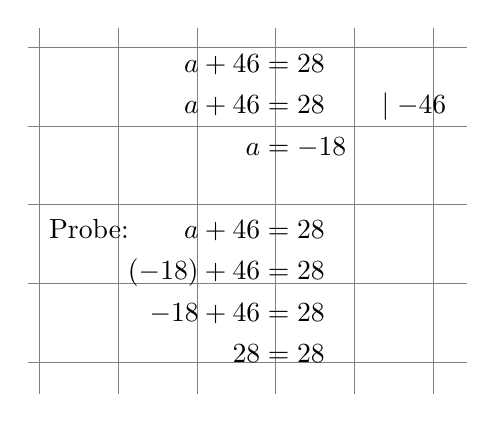
\begin{tikzpicture}[show background grid]
\node[below right] at (0,0.1) {
$\begin{aligned}
a+46  &= 28& &  \\
a + 46 &=28& & \mid - 46\\
a &=-18& & 
\\
\\
\mbox{Probe:}\qquad a+46  &= 28& &  \\
\left(-18\right)+46  &= 28& &  \\
-18+46 &=28& &  \\
28 &=28& &  \\
\end{aligned}$};
\end{tikzpicture}
\endgroup
&
z)&\begingroup\setlength{\jot}{-0.03cm}
\tikzstyle{background grid}=[draw, black!15,step=.5cm]
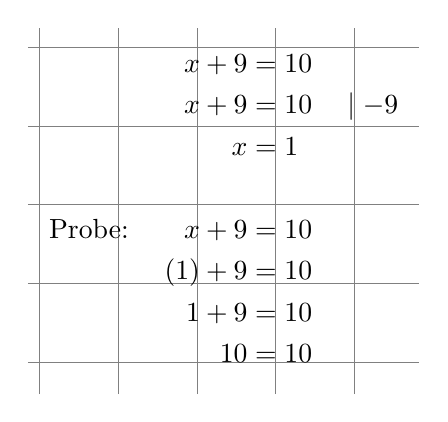
\begin{tikzpicture}[show background grid]
\node[below right] at (0,0.1) {
$\begin{aligned}
x+9  &= 10& &  \\
x + 9 &=10& & \mid - 9\\
x &=1& & 
\\
\\
\mbox{Probe:}\qquad x+9  &= 10& &  \\
\left(1\right)+9  &= 10& &  \\
1+9 &=10& &  \\
10 &=10& &  \\
\end{aligned}$};
\end{tikzpicture}
\endgroup
\\\hline
\end{xltabular}
\vspace{0.5cm}
\end{document}